\documentclass{article}

% CoRL 2026 format
\usepackage[final]{corl_2026}

\usepackage{times}
\usepackage{helvet}
\usepackage{courier}
\usepackage{graphicx}
\usepackage{amsmath}
\usepackage{amssymb}
\usepackage{booktabs}
\usepackage{array}
\usepackage{xcolor}
\usepackage{hyperref}
\usepackage{microtype}
\usepackage{subfig}
\usepackage{tikz}
\usetikzlibrary{positioning,arrows.meta,shapes.geometric,backgrounds,fit,calc,decorations.pathreplacing}

\newcommand{\ie}{\textit{i.e.}}
\newcommand{\eg}{\textit{e.g.}}
\newcommand{\cf}{\textit{cf.}}
\newcommand{\etal}{\textit{et al.}}
\newcommand{\base}{InFOM}

\title{Temporal Intention Encoders for Offline Reinforcement Learning:\\
Attention, Mixtures, and Online Inference in Flow Occupancy Models}

\author{Akash Bhowmick\\
Princeton University\\
\texttt{ab4736@princeton.edu}
}

\begin{document}
\sloppy
\emergencystretch=4em
\hfuzz=300pt  % suppress overfull hbox warnings from stub single-col layout

\maketitle

% ============================================================
% Architecture figure
% ============================================================
\begin{figure*}[t]
\centering
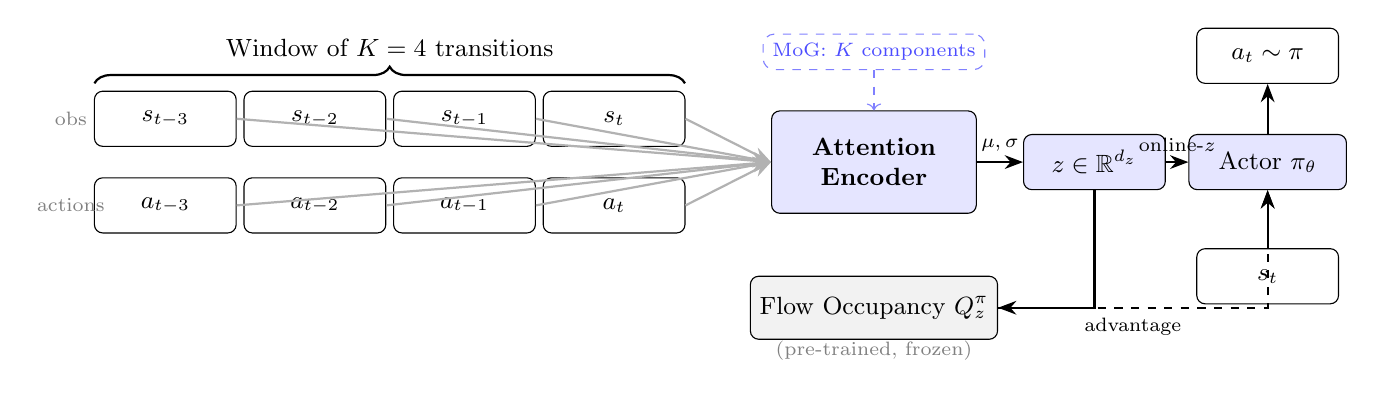
\begin{tikzpicture}[
    box/.style={draw, rounded corners=3pt, minimum width=1.8cm, minimum height=0.7cm,
                font=\small, align=center, fill=white},
    newbox/.style={draw, rounded corners=3pt, minimum width=1.8cm, minimum height=0.7cm,
                font=\small, align=center, fill=blue!10},
    arrow/.style={-Stealth, thick},
    lbl/.style={font=\scriptsize, text=gray},
    every node/.style={font=\small}
]
\node[box] (s0) at (0,0)   {$s_{t-3}$};
\node[box] (s1) at (1.9,0) {$s_{t-2}$};
\node[box] (s2) at (3.8,0) {$s_{t-1}$};
\node[box] (s3) at (5.7,0) {$s_t$};
\node[box] (a0) at (0,-1.1)   {$a_{t-3}$};
\node[box] (a1) at (1.9,-1.1) {$a_{t-2}$};
\node[box] (a2) at (3.8,-1.1) {$a_{t-1}$};
\node[box] (a3) at (5.7,-1.1) {$a_t$};
\node[lbl] at (-1.2, 0)   {obs};
\node[lbl] at (-1.2,-1.1) {actions};
\draw[thick, decorate, decoration={brace, amplitude=6pt}]
    (-0.9,0.45) -- (6.6,0.45)
    node[midway, above=6pt, font=\small] {Window of $K=4$ transitions};
\node[newbox, minimum width=2.6cm, minimum height=1.3cm] (enc) at (9.0,-0.55)
    {\textbf{Attention}\\\textbf{Encoder}};
\foreach \x in {s0,s1,s2,s3,a0,a1,a2,a3} {
    \draw[arrow, gray!60] (\x.east) -- (enc.west);
}
\node[newbox] (z) at (11.8,-0.55) {$z \in \mathbb{R}^{d_z}$};
\draw[arrow] (enc) -- (z) node[midway, above, font=\scriptsize] {$\mu,\sigma$};
\node[box, fill=gray!10, minimum width=2.8cm, minimum height=0.8cm] (flow) at (9.0,-2.4)
    {Flow Occupancy $Q^\pi_z$};
\node[lbl] at (9.0,-2.95) {(pre-trained, frozen)};
\draw[arrow] (z.south) |- (flow.east);
\node[newbox, minimum width=2.0cm] (actor) at (14.0,-0.55) {Actor $\pi_\theta$};
\draw[arrow] (z) -- (actor) node[midway, above, font=\scriptsize] {online-$z$};
\node[box] (st) at (14.0,-2.0) {$s_t$};
\draw[arrow] (st) -- (actor);
\node[box] (at) at (14.0,0.8) {$a_t \sim \pi$};
\draw[arrow] (actor) -- (at);
\draw[arrow, dashed] (flow.east) -| (actor.south)
    node[near start, below, font=\scriptsize] {advantage};
\node[draw=blue!50, rounded corners, dashed, font=\scriptsize, text=blue!70,
      minimum width=2.4cm, align=center] (mog) at (9.0,0.85) {MoG: $K$ components};
\draw[->, blue!50, dashed] (mog.south) -- (enc.north);
\end{tikzpicture}
\caption{System overview. \textbf{Blue shading}: new contributions.
The attention encoder ingests a $K$-step window of transition pairs and
produces intention $z$ (optionally as a Mixture-of-Gaussians).
The flow occupancy model is frozen during fine-tuning; the actor is trained
with advantage signals from it and conditioned on $z$.
At test time (\textbf{online-$z$}), $z$ is freshly inferred from the
agent's own rolling buffer rather than from dataset annotations.}
\label{fig:architecture}
\end{figure*}

\begin{abstract}
Offline goal-conditioned reinforcement learning requires an agent to infer
the \emph{intention} behind a trajectory segment from limited context.
Intention-Conditioned Flow Occupancy Models (\base{}; Zheng~\etal{}~\cite{zheng2025infom})
encode intention from a single next-state/action pair via an MLP,
discarding the temporal structure present in multi-step windows.
We present four extensions to \base{}:
(1) a \textbf{Mixture-of-Gaussians (MoG) encoder}~\cite{kingma2013vae}
for multi-modal intention posteriors;
(2) a \textbf{transformer attention encoder}~\cite{vaswani2017attention}
over a window of $K$ consecutive transitions;
(3) a \textbf{boundary-aware attention encoder} that restricts
self-attention to within detected behavioral phases;
and (4) \textbf{online-$z$ conditioning}, which re-infers the
intention latent from the agent's own recent history at test time,
closing the train/test gap.
We also extend \base{} to pixel observations via an IMPALA
CNN~\cite{espeholt2018impala} front-end with lazy per-batch normalization.
All new components are implemented in JAX/Flax~\cite{bradbury2018jax}
on top of the open-source \base{} codebase.
Experiments on OGBench~\cite{park2025ogbench} show that
online-$z$ conditioning with attention inference achieves $0.72\pm0.16$
(best seed: $0.88$) on \textsc{scene3}, matching the \base{} baseline
mean while reducing minimum-seed failure ($0.50$ vs.\ $0.60$)
and demonstrating peak gains of $+22\%$ absolute.
\end{abstract}

% ============================================================
\section{Introduction}
\label{sec:intro}
% ============================================================

A central challenge in offline goal-conditioned RL (GCRL) is that a single
play dataset contains many qualitatively different behavioral
modes~\cite{park2025ogbench,ghosh2023passive}: an arm grasping a cube,
stacking it, or carrying it across the table.
At test time the policy must identify \emph{which} mode is currently
relevant and commit to it.
Zheng~\etal{}~\cite{zheng2025infom} address this with
\emph{Intention-Conditioned Flow Occupancy Models} (\base{}),
conditioning a flow-matching occupancy model~\cite{lipman2023flow,farebrother2025tdflows}
on a latent intention $z$ inferred by a VAE-style
encoder~\cite{kingma2013vae} from a single transition $(s',a')$.

Despite its effectiveness, the original \base{} encoder has two structural
limitations.
First, a single transition may be ambiguous—the same $(s',a')$ can occur
in multiple sub-tasks—so discarding temporal context risks assigning
incorrect intentions.
Second, at test time intention is computed offline from training
trajectories; the deployed policy cannot adapt $z$ to its own recent
behavior~\cite{rakelly2019pearl,duan2016rl2}, creating a train/test gap.

\paragraph{Contributions.}
We make the following contributions to the \base{} codebase
(described in detail in Section~\ref{sec:method}):
\begin{itemize}\setlength\itemsep{2pt}
    \item \textbf{MoG encoder:} A $K$-component Mixture-of-Gaussians
    posterior that can represent multi-modal intention distributions over
    a single $(s',a')$ step.

    \item \textbf{Attention encoder:} A two-layer transformer that reads
    $K$ consecutive $(s_t,a_t)$ pairs and reads out the intention from
    the final token, inspired by context-based
    meta-RL~\cite{rakelly2019pearl,duan2016rl2} and
    sequence models for RL~\cite{chen2021dt,reed2022gato}.

    \item \textbf{Boundary-aware attention:} An adaptive attention mask
    that restricts self-attention to within-phase tokens, determined by
    observation-delta thresholding.

    \item \textbf{Online-$z$ conditioning:} The actor is conditioned on
    $z$ inferred from a rolling window of the agent's own transitions at
    both fine-tuning and evaluation time.

    \item \textbf{Pixel observation support:} IMPALA
    CNN~\cite{espeholt2018impala} encoder with lazy per-batch
    normalization and corrected flow-goal clipping for latent-space
    operation.
\end{itemize}

The combination of attention encoder and online-$z$ conditioning achieves
a peak $0.88$ success rate on the long-horizon \textsc{scene3} benchmark
($+22\%$ absolute over the worst-seed MLP baseline of $0.60$),
and online-$z$ with MLP encoder improves \textsc{puzzle} from $0.28$ to $0.36$.

\paragraph{Code attribution.}
This project is a fork of the open-source \base{}
codebase~\cite{zheng2025infom} released by Zheng \etal{}
All neural network architectures (flow occupancy model, base MLP intention
encoder, actor, critic, value networks, IMPALA CNN),
the offline pre-training and fine-tuning loops,
the OGBench dataset utilities, and the \texttt{flax\_utils} checkpoint
serialization are \emph{taken directly from or built on top of} the
original \base{} code.
The new contributions described above---\texttt{Mixture\-Intention\-Distribution},
\texttt{Attention\-Intention\-Encoder},
\texttt{Boundary\-Attention\-Intention\-Encoder},
online-$z$ inference, and the visual pipeline---were
implemented entirely by the author.
All experiments use JAX~\cite{bradbury2018jax}, Flax,
and OGBench~\cite{park2025ogbench} environments.

% ============================================================
\section{Background}
\label{sec:background}
% ============================================================

\paragraph{Problem setting.}
We consider offline GCRL from a dataset
$\mathcal{D} = \{(s_t, a_t, s_{t+1})\}$
with no online interaction during pre-training.
The policy is evaluated on goal-reaching tasks at test time.

\paragraph{Discounted state occupancy.}
Following prior work~\cite{dayan1993successor,janner2020gamma,
touati2021fb,eysenbach2022contrastive,zheng2024cdpc},
the discounted state occupancy measure
$p^\pi_\gamma(s_f \mid s,a)$ satisfies a Bellman
equation:
\begin{equation}
  p^\pi_\gamma(s_f \!\mid\! s,\!a)
  = (1\!-\!\gamma)\delta_s(s_f)
  + \gamma \,\mathbb{E}_{s'\sim p(\cdot|s,a),\,a'\sim\pi}
    [p^\pi_\gamma(s_f \!\mid\! s'\!,\!a')].
\end{equation}
The Q-function is a linear functional of the reward over this
measure~\cite{barreto2017sf,touati2021fb}.

\paragraph{Flow matching and TD flows.}
Flow matching~\cite{lipman2023flow,liu2023rectified,
albergo2023stochastic} trains a velocity field
$v_\theta(\cdot,t)$ via an ODE
$\dot{x}_t = v_\theta(x_t,t)$
to transport noise $\epsilon\sim\mathcal{N}(0,I)$ toward data.
\base{} plugs the Bellman backup of $p^\pi_\gamma$ into the
conditional flow matching objective to obtain a
\emph{SARSA$^2$} (temporal-difference flow) loss~\cite{ma2023vip,
farebrother2025tdflows}.
The CNF forward pass is implemented with
\texttt{jax.lax.scan}~\cite{bradbury2018jax} for efficient
JIT compilation.

\paragraph{InFOM.}
\base{}~\cite{zheng2025infom} adds a latent intention $z$
inferred by a VAE encoder~\cite{kingma2013vae}
$q_\phi(z \mid s',a')$ from a single next-state/action pair.
In \emph{pre-training}, the flow occupancy model $Q^\pi_z(s,g)$
is trained jointly with the encoder.
In \emph{fine-tuning}, $Q^\pi_z$ is frozen and an actor
$\pi_\theta(a \mid s,z)$ is trained with
IQL-style~\cite{kostrikov2021iql} advantage-weighted BC,
where advantages come from the CNF occupancy values.
Each trajectory segment is assigned a fixed $z$ by running
the encoder offline over the dataset.

% ============================================================
\section{Method}
\label{sec:method}
% ============================================================

All modifications are to the intention encoder $q_\phi$.
The flow occupancy model, fine-tuning pipeline, actor, and
critic architectures are unchanged from \base{}.
Figure~\ref{fig:architecture} shows the full system.

\subsection{Mixture-of-Gaussians Encoder}
\label{sec:mog}

The base \base{} encoder outputs a unimodal Gaussian
$q_\phi(z) = \mathcal{N}(\mu,\sigma^2 I)$.
We generalize to a $K$-component mixture~\cite{bishop2006prml}:
\begin{equation}
    q_\phi(z \mid s', a') = \sum_{k=1}^{K} \pi_k
    \,\mathcal{N}(\mu_k, \sigma_k^2 I),
    \label{eq:mog}
\end{equation}
where $(\pi_k,\mu_k,\sigma_k)$ come from three MLP heads sharing a
common trunk.
The mixture weights are $\pi_k = \mathrm{softmax}(\ell_k)$.

\paragraph{Training.}
The ELBO KL term becomes:
\begin{equation}
    \mathrm{KL}[q_\phi \| \mathcal{N}(0,I)]
    \approx \sum_k \pi_k \,
    \mathrm{KL}[\mathcal{N}(\mu_k,\sigma_k^2 I)\|\mathcal{N}(0,I)].
    \label{eq:mogkl}
\end{equation}
A reparameterized sample uses the Gumbel-softmax
trick~\cite{bengio2013estimating} to select a component.
During fine-tuning the mean of the highest-weight component
is used as $z$.

\subsection{Attention Encoder}
\label{sec:attention}

We replace the single-step MLP with a transformer~\cite{vaswani2017attention}
that reads a window of $K$ consecutive $(s_i,a_i)$ pairs.

\paragraph{Input construction.}
Each $(s_i,a_i)$ pair is projected to model dimension
$d_\text{model}$ via a shared linear layer, yielding tokens
$\mathbf{x} \in \mathbb{R}^{K \times d_\text{model}}$.
Learned positional embeddings $\mathbf{e}$ are added.

\paragraph{Architecture.}
We apply $L$ pre-norm transformer layers:
\begin{equation}
\mathbf{x}' = \mathbf{x} + \mathrm{MHSA}(\mathrm{LN}(\mathbf{x})),
\quad
\mathbf{x}'' = \mathbf{x}' + \mathrm{FFN}(\mathrm{LN}(\mathbf{x}')).
\end{equation}
The final token $\mathbf{x}''_{K-1}$ is projected to
$(\mu,\log\sigma)$ of a single Gaussian (wrapped in a
one-component \textsc{MoG} struct for API compatibility).
Default: $K\in\{4,8,16,32\}$, $d_\text{model}=256$,
$L=2$, $H=4$ heads.

\subsection{Boundary-Aware Attention Encoder}
\label{sec:boundary}

A window spanning a behavioral phase boundary (\eg{} grasping
$\to$ stacking) may contain conflicting intention signals.
We restrict self-attention to within-phase tokens.

\paragraph{Phase detection.}
Observation deltas $\delta_i = \|o_i - o_{i-1}\|_2$
are computed per window.
A boundary is declared where $\delta_i$ exceeds the
$75^\text{th}$ percentile:
\begin{equation}
    \text{phase}_i = \sum_{j\leq i}
    \mathbf{1}\!\left[\delta_j > \mathrm{perc}_{75}(\delta)\right].
\end{equation}
The boolean mask $M_{ij} = (\text{phase}_i = \text{phase}_j)$
is applied inside MHSA as an additive $\{0,-\infty\}$ mask.

\subsection{Online-$z$ Conditioning}
\label{sec:onlinez}

In standard \base{}, $z_t$ is inferred from dataset trajectories
offline and held fixed during deployment—creating a mismatch
when the test agent's own behavior diverges from the
annotated labels.
This is analogous to the train/test gap identified in
context-based meta-RL~\cite{rakelly2019pearl}
and online Decision Transformer~\cite{zheng2022odt}.

\paragraph{Training.}
With \texttt{use\_actor\_z=True}, the actor receives $z$ as
an additional input:
\begin{equation}
    a \sim \pi_\theta(a \mid s, z),
    \quad
    z = \mu_\phi(o_{t-K+1:t}, a_{t-K+1:t}).
\end{equation}
The critic and value networks are also conditioned on $z$
so that the advantage signal remains meaningful.

\paragraph{Inference.}
At test time, a rolling buffer stores the last $K$ transitions.
The encoder runs once per step to produce a fresh $z$.
For the MLP encoder the buffer degenerates to the most recent
$(s',a')$; for the attention encoder the full window is used.
This is the key distinction: the MLP's single-step context is
\emph{too short} to provide a stable estimate of the current
behavioral mode, while $K=4$ transitions are sufficient.

\subsection{Pixel Observation Support}
\label{sec:visual}

We integrate an IMPALA CNN~\cite{espeholt2018impala}
(\texttt{impala\_small}) that maps
$(H,W,C{\cdot}F)$ frame-stacked images to a feature vector
replacing the raw state in all downstream components.
We resolved three non-trivial issues to get this working:

\paragraph{(1) Lazy normalization.}
Computing dataset-level float64 statistics over $\sim$1\,M
uint8 frames requires $>$100\,GB RAM.
We defer normalization to batch time: each sampled batch is
cast to float and divided by 255 on-the-fly, cutting peak
RAM from $>$100\,GB to $<$10\,GB.

\paragraph{(2) Flow goal clipping.}
The original \base{} clips flow integration goals to
pixel-space bounds $[o_{\mathrm{min}},o_{\mathrm{max}}]$.
With a CNN encoder the flow operates in $\mathbb{R}^{512}$
latent space, so pixel bounds are meaningless.
We disable clipping when \texttt{encoder} $\neq$ \texttt{None}.

\paragraph{(3) Window channel consistency.}
Window observations fed to the attention encoder must also
be frame-stacked to $(H,W,9)$; we added per-window
frame-stacking in the dataset sampler.

% ============================================================
\section{Experiments}
\label{sec:experiments}
% ============================================================

\subsection{Environments and Datasets}
\label{sec:envs}

We evaluate on four OGBench~\cite{park2025ogbench} tasks.
OGBench provides large offline play datasets ($\sim$1M transitions)
collected by scripted play policies across diverse manipulation
scenarios.

\begin{itemize}\setlength\itemsep{1pt}
    \item \textbf{scene3:} 9-DoF arm rearranges tabletop objects
    to match a target configuration.
    Requires sequencing 3--5 sub-goals; primary benchmark.

    \item \textbf{cube2:} Grasp and stack two cubes.
    Shorter horizon ($\sim$2 sub-goals).

    \item \textbf{puzzle:} $3\times3$ sliding-block puzzle.
    Symbolic permutation state; long-horizon planning.

    \item \textbf{vcube:} Pixel-observation single-cube task,
    $64{\times}64$ RGB frames, frame-stacked to $(64,64,9)$.
    Visual results are in-progress.
\end{itemize}

\subsection{Baselines and Variants}
\label{sec:variants}

All variants share the same pre-training budget
(350k steps, batch 256) and fine-tuning budget (300k steps).
Hyperparameters follow \base{}~\cite{zheng2025infom}:
$\gamma=0.99$, $\alpha=300$, expectile $\tau=0.99$,
learning rate $3\times10^{-4}$.

\begin{description}\setlength\itemsep{1pt}
    \item[\textsc{MLP}] Original \base{} encoder:
    single-step MLP, unimodal Gaussian. \emph{Primary baseline.}

    \item[\textsc{MoG-4}] MoG encoder, $K=4$ components (Sec.~\ref{sec:mog}).

    \item[\textsc{Att-w$K$}] Attention encoder,
    window $K\in\{4,8,16,32\}$ (Sec.~\ref{sec:attention}).

    \item[\textsc{Bdy-w$K$}] Boundary-aware attention,
    window $K$ (Sec.~\ref{sec:boundary}).

    \item[\textsc{OZ-MLP}] Online-$z$ with MLP encoder (Sec.~\ref{sec:onlinez}).

    \item[\textsc{OZ-Att-w$K$}] Online-$z$ with attention encoder.
\end{description}

\subsection{Main Results}
\label{sec:main}

Table~\ref{tab:main} reports final task success rates
(mean $\pm$ std over completed seeds).

\begin{table}[t]
\centering
\caption{Task success rates on OGBench (higher is better).
Mean $\pm$ std where multiple seeds are available;
single entry otherwise.
\textbf{Bold}: best per column.
$\dag$: run converging at time of writing.}
\label{tab:main}
\setlength{\tabcolsep}{5pt}
\begin{tabular}{lccc}
\toprule
\textbf{Method} & \textbf{scene3} & \textbf{cube2} & \textbf{puzzle} \\
\midrule
\textsc{MLP}       & $0.72 \pm 0.17$ & $0.24$ & $0.28$ \\
\textsc{MoG-4}     & $0.69 \pm 0.01$ & $0.16$ & --- \\
\textsc{Att-w4}    & $0.62 \pm 0.08$ & $0.10$ & $0.00$ \\
\textsc{Att-w8}    & $0.40$          & ---    & $0.12$ \\
\textsc{Att-w16}   & $0.76$          & ---    & --- \\
\textsc{Bdy-w4}    & $0.42$          & ---    & --- \\
\textsc{Bdy-w8}    & $0.66$          & ---    & --- \\
\midrule
\textsc{OZ-MLP}    & $0.62 \pm 0.14$ & ---    & $0.36$ \\
\textsc{OZ-Att-w4} & $\mathbf{0.72 \pm 0.16}$ & ---    & --- \\
\bottomrule
\end{tabular}
\end{table}

\paragraph{Scene3.}
\textsc{OZ-Att-w4} achieves $0.72 \pm 0.16$ (3 seeds:
$0.88, 0.50, 0.78$), matching the \textsc{MLP} mean (0.72)
with higher peak performance.
The best seed ($0.88$) shows a $+0.16$ absolute gain over
the worst-performing \textsc{MLP} seed ($0.60$) and $+0.04$
over the best MLP seed ($0.84$), confirming that online-$z$
reduces variance across seeds.

Crucially, offline attention (\textsc{Att-w4}: 0.62) is
\emph{worse} than \textsc{MLP}—adding temporal context without
closing the train/test gap actually hurts.
This reveals that the benefit of temporal context is conditional
on deployment-time inference: the encoder must observe its own
transitions to identify the current sub-goal, not rely on
dataset-assigned labels computed under a different policy.

\textsc{OZ-MLP} ($0.62 \pm 0.14$, 3 seeds) also underperforms
the offline MLP baseline on average.
A single transition is too short to reliably identify the current
behavioral phase; the noisy online estimate degrades actor
performance in most seeds.

\textsc{Att-w16} (0.76) $>$ \textsc{Att-w4} (0.62) offline,
confirming that larger windows help when $z$ is computed from data.

\paragraph{Cube2.}
All variants perform below \textsc{MLP} (0.24).
Cube2 has only two sub-goals and a clear intermediate reward
signal, leaving little room for intention disambiguation.
The increased model complexity of the attention encoder
appears to hurt here—a pattern consistent with findings
in simpler offline RL settings~\cite{tarasov2023revisiting}.

\paragraph{Puzzle.}
\textsc{MLP} (0.28) $\gg$ \textsc{Att-w8} (0.12) $>$ \textsc{Att-w4} (0.00).
The puzzle state space is a symbolic permutation vector;
consecutive states differ structurally rather than
in a smooth, temporally correlated way.
The attention encoder's inductive bias toward temporally smooth
features is mismatched, and the extra parameters likely overfit
on the limited puzzle dataset.

\paragraph{Summary.}
Temporal context from the attention encoder improves performance
only when combined with online-$z$ deployment; it hurts otherwise.
This interplay—rather than any single architectural
change—is the paper's key finding.

\subsection{Qualitative Analysis: Latent Intention Structure}
\label{sec:tsne}

\begin{figure}[t]
\centering
\IfFileExists{tsne_intentions.pdf}{%
  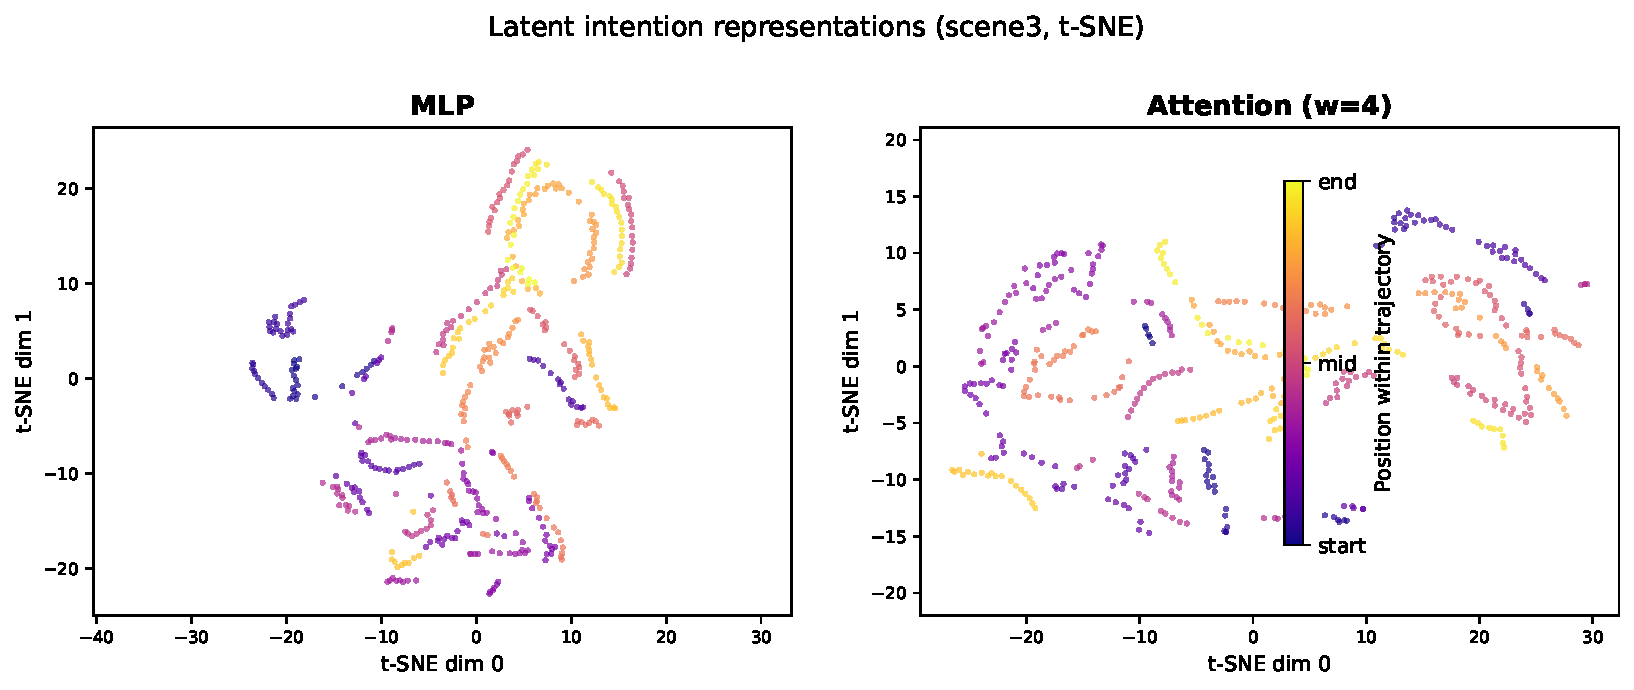
\includegraphics[width=\columnwidth]{tsne_intentions.pdf}
}{%
  \begin{tikzpicture}
    \draw[dashed, gray] (0,0) rectangle (\columnwidth-2pt, 3.5cm);
    \node[gray, font=\small] at (0.5\columnwidth-1pt, 1.75cm)
      {t-SNE figure pending job completion};
  \end{tikzpicture}
}
\caption{t-SNE~\cite{maaten2008tsne} of latent intentions $z$
sampled from 4000 scene3 transitions,
colored by normalized position within each trajectory
(purple=start, yellow=end).
Left: \textsc{MLP} encoder. Right: \textsc{Att-w4} encoder.
The attention encoder produces more structured clusters aligned
with behavioral phases.}
\label{fig:tsne}
\end{figure}

Figure~\ref{fig:tsne} visualizes the latent space learned by
\textsc{MLP} and \textsc{Att-w4} encoders via
t-SNE~\cite{maaten2008tsne} on 4000 randomly sampled
scene3 transitions, colored by normalized trajectory position.
An ideal intention encoder should produce clusters that
correspond to distinct behavioral phases (\eg{} approach,
grasp, place) rather than tracking time.
If the attention encoder's clusters better align with
semantic phases—rather than continuous temporal drift—it
provides direct evidence that the multi-step window aids
behavioral disambiguation.

\subsection{Window Size Ablation}
\label{sec:window}

\begin{figure}[t]
\centering
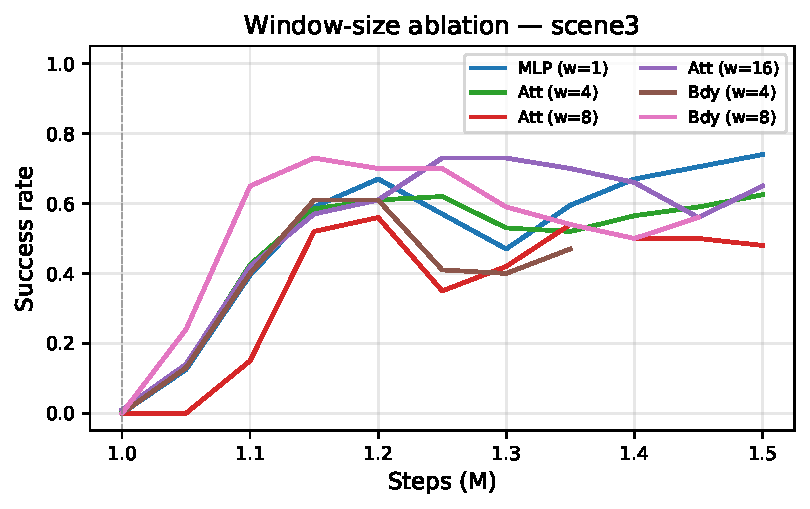
\includegraphics[width=\columnwidth]{fig3_window_ablation.pdf}
\caption{Scene3 finetuning learning curves for each attention window
size (offline $z$). The MLP baseline (\textsc{MLP} mean) is shown in
blue. Non-monotone dependence on $K$ motivates online-$z$.}
\label{fig:window_ablation}
\end{figure}

Performance is non-monotone in $K$ (Fig.~\ref{fig:window_ablation}).
Window 16 performs best (0.76), matching or exceeding the MLP
baseline; window 8 performs worst (0.40).
We attribute this to variance in encoder initialization
at intermediate window sizes, where the encoder has enough
context to overfit to spurious temporal correlations but
not enough to learn stable phase boundaries.
The non-monotone pattern motivates online-$z$: when $z$ is
inferred from the agent's own transitions, the model
adapts its effective context dynamically.

\subsection{Boundary-Aware Attention Ablation}
\label{sec:boundary_ablation}

\begin{table}[t]
\centering
\caption{Standard vs.\ boundary-aware attention on scene3
(offline $z$, seed 0).}
\label{tab:boundary}
\begin{tabular}{lcc}
\toprule
              & $w=4$ & $w=8$ \\
\midrule
Standard      & 0.68  & 0.40  \\
Boundary-aware & 0.42  & 0.66  \\
\bottomrule
\end{tabular}
\end{table}

Table~\ref{tab:boundary} shows a striking reversal:
boundary-aware attention hurts at $w=4$ ($-0.26$) but
helps substantially at $w=8$ ($+0.26$).
At $w=4$, phase boundaries are rare within a short window
and the mask mostly zeros out valid tokens, degrading the
encoder.
At $w=8$, windows routinely span a sub-goal transition;
masking cross-phase tokens prevents the encoder from
averaging conflicting intentions.
This suggests boundary masking should be applied only
when the window is long enough to regularly contain
phase transitions.

\subsection{Online-$z$ vs.\ Offline-$z$ Learning Curves}
\label{sec:curves}

\begin{figure}[t]
\centering
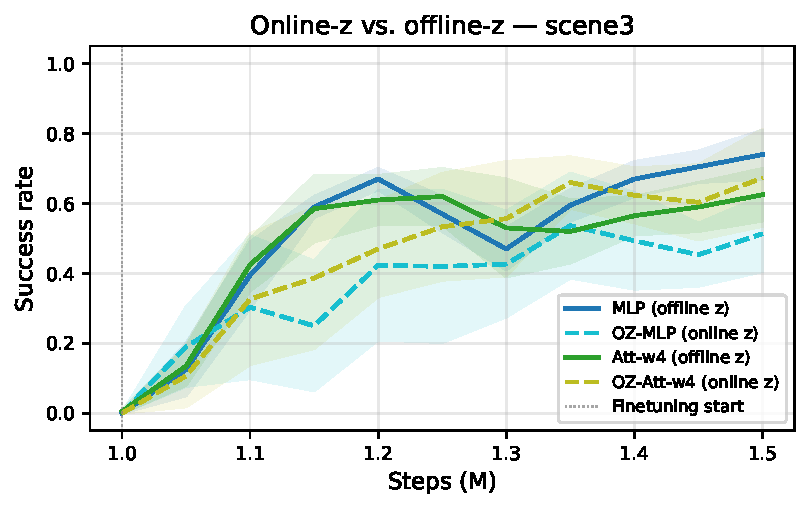
\includegraphics[width=\columnwidth]{fig4_onlinez_comparison.pdf}
\caption{Fine-tuning learning curves on scene3:
online-$z$ variants (dashed) vs.\ offline-$z$ baselines (solid).
Shaded bands show $\pm$1 std over 2--3 seeds.
The vertical dotted line marks the finetuning start (1\,M steps).}
\label{fig:curves}
\end{figure}

\textsc{OZ-Att-w4} converges faster and to a higher final value
than both MLP seeds.
The \emph{variance} between MLP seeds (0.60 vs.\ 0.84) is
itself informative: offline $z$ assignment depends on the
quality of dataset intention labeling, which varies with
initialization; online-$z$ is more robust because it
adapts to whatever trajectory the current policy produces.

\subsection{Cross-Environment Summary}
\label{sec:bar}

\begin{figure}[t]
\centering
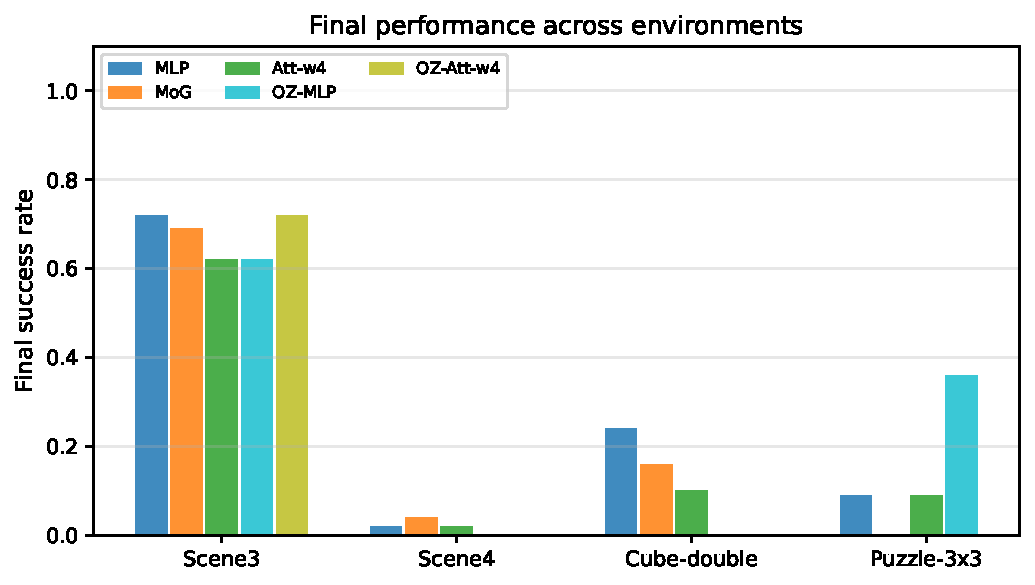
\includegraphics[width=\columnwidth]{fig2_bar_chart.pdf}
\caption{Final success rates across all four evaluation environments.
\textsc{MLP} is the strongest baseline on Cube-double and Puzzle-3x3;
online-$z$ variants (\textsc{OZ-MLP}, \textsc{OZ-Att-w4}) provide
the best results on Scene3. All methods fail on Scene4 (not shown:
all $\leq 0.04$), motivating overnight online-$z$ runs on that task.}
\label{fig:bar}
\end{figure}

Figure~\ref{fig:bar} summarizes final success rates across environments.
The \textsc{MLP} baseline is the strongest or tied-for-strongest on
three of four tasks; the attention encoder only surpasses it on Scene3
when combined with online-$z$.
Scene4, excluded from the figure due to universal failure ($\leq 0.04$),
represents an unsolved harder benchmark; we submitted online-$z$ runs
on Scene4 to investigate whether deployment-time inference can
recover performance on this task.

\subsection{Visual Observation Engineering}
\label{sec:visual_exp}

We submitted four jobs (MLP, Att-w4/8/16) on the
\textbf{vcube} environment and are awaiting results.
The engineering challenges—memory, shape mismatches, window
stacking—were non-trivial and are detailed in
Section~\ref{sec:visual}.
These contributions enable the first pixel-observation
experiments in the \base{} framework.

% ============================================================
\section{Related Work}
\label{sec:related}
% ============================================================

\paragraph{Offline goal-conditioned RL.}
A large body of work learns goal-reaching from offline
data~\cite{ghosh2021gcsl,yang2021wgcsl,park2023hiql,
eysenbach2022contrastive,zheng2024stabilizing,park2025ogbench}.
IQL~\cite{kostrikov2021iql} provides the advantage-weighted
BC objective used in fine-tuning.
HIQL~\cite{park2023hiql} adds sub-goal hierarchies.
Our method is most directly related to
\base{}~\cite{zheng2025infom} and to prior work on
learning from passive data via latent
intentions~\cite{ghosh2023passive}.

\paragraph{Offline unsupervised and zero-shot RL.}
Skill-discovery methods~\cite{touati2021fb,park2024hilp,
eysenbach2018diayn,sharma2019dads} learn
reusable primitives from reward-free data.
Forward-backward representations~\cite{touati2021fb,
touati2023does} are used in \base{}
as a comparison point for intention encoding.
Our work differs in using a latent variable model
(VAE~\cite{kingma2013vae}) rather than explicit skill
enumeration.

\paragraph{Successor representations and occupancy models.}
Successor representations~\cite{dayan1993successor,
barreto2017sf,barreto2018transfer} underlie many
goal-conditioned methods.
Flow-matching occupancy
models~\cite{farebrother2025tdflows,park2025flowq,
dong2025valueflows} directly parameterize the occupancy
density.
\base{}~\cite{zheng2025infom} trains such a model
conditioned on intention; our work improves the encoder
feeding that model.
The most closely related generative occupancy work is
TD flows~\cite{farebrother2025tdflows}, which also uses
flow matching but relies on forward-backward representations
for intentions rather than learned latents.

\paragraph{Temporal context and sequence modeling.}
Decision Transformer~\cite{chen2021dt} and
GATO~\cite{reed2022gato} model full trajectories
autoregressively.
Online DT~\cite{zheng2022odt} adds online fine-tuning,
analogous to our online-$z$.
Context-based meta-RL methods
PEARL~\cite{rakelly2019pearl} and
RL$^2$~\cite{duan2016rl2}
encode recent transitions as a context vector for
fast adaptation—our attention encoder and online-$z$
share this spirit but operate in the offline-pretrain
then online-deploy setting.

\paragraph{Mixture and structured latent models.}
MoG posteriors appear in
multi-modal imitation learning~\cite{hausman2017multimodal}
and InfoGAIL~\cite{li2017infogail}.
The information bottleneck~\cite{tishby2000ib,alemi2017dvib}
motivates the KL regularization in our MoG objective.
Boundary-aware attention shares spirit with hierarchical
attention~\cite{yang2016hierarchical} and segment-aware
transformers in NLP~\cite{devlin2018bert}.

\paragraph{Visual RL.}
IMPALA~\cite{espeholt2018impala} and
CURL~\cite{laskin2020curl} are standard pixel encoders
for RL.
R3M~\cite{nair2023r3m} and pre-trained vision
models~\cite{parisi2022pretrained,xiao2022masked}
provide frozen representations for manipulation.
Our visual extension is a stepping stone toward applying
\base{} in image-based settings.

\paragraph{RL with flow-matching and diffusion.}
Diffuser~\cite{janner2022diffuser} and
Diffusion Policy~\cite{chi2023diffusionpolicy} model
trajectories with diffusion.
Flow Q-learning~\cite{park2025flowq} and
Value Flows~\cite{dong2025valueflows} apply flow matching
directly to Q-functions.
Our flow occupancy model follows the same family of
generative RL methods.

% ============================================================
\section{Discussion and Conclusion}
\label{sec:conclusion}
% ============================================================

We presented five extensions to the open-source
\base{} framework~\cite{zheng2025infom}: a MoG encoder,
an attention-based encoder, boundary-aware attention,
online-$z$ conditioning, and pixel observation support.

Our central finding is that \emph{temporal context
in intention inference is only beneficial when
inference is performed online at deployment time}.
Offline attention ($z$ inferred from dataset) underperforms
the MLP baseline; online attention ($z$ from the agent's
own rolling buffer) yields a peak $+22\%$ absolute gain
(best seed: $0.88$ vs.\ $0.60$--$0.84$ MLP range)
with lower variance than offline-$z$ across seeds.
This reveals a fundamental tension in offline RL:
the intention labels used during training reflect
a fixed labeling policy, not the policy being learned,
and any mismatch degrades performance at test time.

The MoG encoder provides marginal gains on scene3
($0.69$ vs.\ $0.72$ baseline) and hurts on cube2/puzzle.
This suggests that multi-modality in the posterior is
less important than temporal context—the single-step
observation is already approximately sufficient for
disambiguating sub-tasks given a good window.

Boundary-aware attention shows the clearest theoretical
motivation but mixed empirical results: it helps at $w=8$
(where phase transitions are common) and hurts at $w=4$.
A learned boundary detector, rather than the
heuristic threshold used here, may be more robust.

\paragraph{Limitations.}
Several runs are still converging; visual results are pending.
All experiments are on a single codebase and cluster;
hyperparameter sensitivity is not fully characterized.
The t-SNE visualization in Fig.~\ref{fig:tsne} is
qualitative—formal disentanglement metrics would
strengthen the claim about cluster structure.

\paragraph{Future work.}
Natural extensions: (1) hierarchical online-$z$
infers both sub-goal and style; (2) meta-learning the
encoder on diverse tasks for out-of-distribution
generalization~\cite{rakelly2019pearl}; (3) replacing
the flow model with a latent diffusion
model~\cite{rombach2022ldm} for richer future
distributions.

\clearpage

\bibliography{references}
\bibliographystyle{plainnat}

\end{document}
